%
% File: chap02.tex
% Author: Oliver J. H. Feighan
% Description: delta-scf benchmarking, including dft and dftb methods.
% Talk about important factors for modelling LHII
%
\let\textcircled=\pgftextcircled
\chapter{Mean-Field excited states}
\label{chap:dscf}

\initial {P}reamble

%=======
\section{Theory}
\label{sec:dscf_theory}

\subsection{$\Delta$-SCF and eigenvalue difference}
\label{subsec{dscf_and_eigdiff}}

\dscf predicts the excitation energy of a system by comparing the single point
energy of the ground state and the excited state. Finding this excited state
correctly can be an issue, but is usually assumed to be similar to the ground
state. In its simplest form, the \dscf method calculates the ground state, and
then calculates the excited state by rerunning an self-consistent field (SCF) 
with the excited state occupation numbers. This then gives a full description 
of both the ground as excited state from the orbital coefficients output from 
the two SCF procedures.

Initially, the excited state could be calculated by relaxing the orbitals which
contain the excited electron and hole in the ground state space, so that the
excited state and ground state are orthogonal\cite{Hunt1969}. However, it was
argued that this procedure would exacerbate errors from finding the ground
state, and that the excited state was not a proper SCF solution\cite{Gilbert2008}.
Alternatively, it was proposed that an SCF like method, where instead of
populating orbitals according to the aufbau principle, orbitals which most
resemble the previous iteration's orbitals should be occupied. Each iteration 
in an SCF procedure produces new molecular orbital coefficients by solving the 
Roothaan-Hall equations\cite{Roothaan1951}, generally given as an eigenvalue problem:

\begin{equation}
\mathbf{F} \mathbf{C}^{\text{new}} = \mathbf{S} \mathbf{C}^{\text{new}} \epsilon
\end{equation}

where $\mathbf{C}^{\text{new}}$ are the next orbital coefficient solutions, 
$\mathbf{S}$ is the overlap, and $\epsilon$ are the orbital energies. 
The Fock matrix $\mathbf{F}$ is calculated from the previous set of orbital 
coefficients:

\begin{equation}
\mathbf{F} = f\left(\mathbf{C}^{\text{old}}\right)
\end{equation}

The amount of similarity of orbitals can be estimated from their overlap:

\begin{equation}
\mathbf{O} = \left(\mathbf{C}^{\text{old}}\right)^\dagger \mathbf{S} \mathbf{C}^{\text{new}}
\end{equation}

and for a single orbital can be evaluated as a projection:

\begin{equation}
p_j = \sum^n_i O_{ij} = \sum^N_\nu \left[\sum^N_\mu\left(\sum^n_i C_{i\mu}^{\text{old}}\right)S_{\mu\nu}\right]C^{\text{new}}_{\nu j}
\end{equation}

where $\mu,\nu$ are orbital indices. The population can then be given by the set
of orbitals with the highest projection $p_j$.  This method can be used for any
excited state, with the caveat that the orbital solution is in the same region
as the ground state solution. For a few low lying states, this is generally 
true, and so \dscf can be used to calculate a spectrum of excited states\cite{Gilbert2008}.
The method of using this orbital overlap is called the maximum overlap method (MOM).

\dscf has been shown to be cheap alternative to TDDFT and other higher level
methods, without considerable losses of accuracy in certain cases\cite{Worster2021}.
Additionally, as the excited state is given as solutions to SCF equations,
the gradient of this solution can be given by normal mean-field theory.
These gradients would be much cheaper than TDDFT or coupled cluster methods, and
so would be advantageous for a dynamic simulation of LHII.

The final descent in response theory would be to eigenvalue difference methods. 
Here there is assumed to be no response of the orbital energies and shapes when 
interacting with light. As stated earlier, this would be recovered from the
complete Cassida equation if the coupling elements in the $\mathbf{A}$ and 
$\mathbf{B}$ matrices are set to zero. This means that the difference between 
the excited state energy and the ground state energy is just the difference of
the orbital energies between the orbital an electron has been excited to and the
orbital has been excited from. Additionally, transition properties can be 
calculated by calculating transition density matrices from only the ground state.
Hence, all the information needed can be given by a single SCF optimization. 
Generally, eigenvalue difference methods are not seen as accurate response methods,
but can offer a quick and easy initial value\cite{Gimon2009}.

\subsection{Semi-empirical extensions}
\label{subsec:dscf_xtb}
We tried to extend the range of DFT methods that could be used for \dscf and 
eigenvalue difference methods by investigating whether a tight-binding method
could predict transition properties.
We chose the recently published DFTB method parameterized by the Grimme group for
this. This method has been parameterized for geometries, frequencies and non-covalent
interactions, and uses an extended version of H{\"u}ckel theory. The name they
present is GFN-xTB, standing for "Geometries, Frequencies, Non-Covalent - eXtended 
Tight Binding".
We chose this method for two reasons. The first being that the GFN-xTB method was
already implemented in the \code{QCORE} package. This significantly reduced the
amount of effort required for this project. Additionally, there would be other
users and developers who would help with implementation of this new method.
The second, more scientific reason, is that a similar method has already been
published that calculates transition properties. This is the sTDA-xTB method. 
As this method has similar goals as this project, it is useful to look at this 
in more detail.

\subsubsection{sTDA-xTB}
\label{subsubsec:stda_xtb}
A similar method to GFN1-xTB has already shown to be accurate at predicting
transition properties for large systems, with exceptional speed. This method was
published as the sTDA-xTB method\cite{Grimme2016}. The drop in accuracy for this
method is minimal, with the error being around 0.3 - 0.5 eV.

Similar to other xTB methods, the sTDA-xTB method is a tight-binding method that
uses empirically fit parameters and a minimal basis set. It was trained on a
test set of highly accurate coupled cluster and density functional theory
excitation energies, as well as accurate atomic partial charges.

Unlike other xTB methods, the basis set for sTDA-xTB is dependent on the D3
coordination number. This makes this method far more flexible, which would usually
be achieved in a fixed basis set by using diffuse or else additional orbitals in
the basis set. Additionally, it uses two sets of parameterized basis sets - a
smaller valence basis set (VBS) and an extended basis set (XBS).

These two basis sets are used to construct formally similar Fock matrix elements,
however in practice these use different global parameters. The core Hamiltonian
is similar to other DFTB methods that use a self-consistent charge method, as
opposed to an SCF method, to obtain molecular orbital coefficients. It is given by:

\begin{equation}
\bra{\psi_\mu} H^{\text{EHT, sTDA-xTB}} \ket{\psi_\mu}= \frac{1}{2} \left(k^l_\mu k^{l'}_\nu\right) \frac{1}{2} \left(h^l_\mu h^{l'}_\nu\right) S_{\mu\nu} - k_T \bra{\psi_\mu}\hat{T}\ket{\psi_\nu}
\end{equation}

where, $\mu,\nu,l,l'$ are orbital and shell indices  $k^l_\mu$ are shell-wise 
H{\"u}ckel parameters, $h$ are effective atomic-orbital energy levels, $S$ is
the overlap, $k_T$ is a global constant and $\hat{T}$ is the kinetic energy 
operator. The charges used in the inter-electronic repulsion function are given 
by CM5 charges for the XBS Fock matrix. These are calculated using Mulliken 
charges obtained from diagonalising the Fock matrix with the VBS. The charges for 
the initial VBS Fock matrix are based on Gasteiger charges, modified by the 
electronegativities of atoms in the system.

The whole process for determining molecular orbitals can be summarized as:
\begin{enumerate}
	\item Calculate modified Gasteiger charges for initial guess
	\item Diagonalize Fock matrix in the VBS to get the first set of Mulliken charges
	\item Compute CM5 charges
	\item Diagonalize Fock matrix in the VBS again for final set of Mulliken charges.
	\item Recalculate CM5 charges with this final set, and diagonalize the Fock matrix in the XBS. The molecular orbital coefficients from this are then fed to the response theory.
\end{enumerate}

The response theory for this method is based on the previous work in the Grimme 
group on the simplified Tann-Dancoff Approximation. There are several approximations 
made between full linear response theory and the sTDA method. First is the 
Tann-Danncoff approximation, where the B matrix is ignored. The second approximation 
is to use Mataga-Nishimoto-Ohno-Klopman (MNOK) integrals instead of explicit 2 electron 
integrals to calculate matrix elements, as well as neglecting the density 
functional term. 

Transition charges are used to calculate these MNOK integrals, where the charges 
are computed using a Löwdin population analysis. The operator is the 
MNOK\cite{Nishimoto1957}\cite{Ohno1964}\cite{Klopman1964} damped coloub function, 
with different exponents $y_K$ and $j_J$ for exchange and coulomb integral respectively. 
The $a_x$ parameter is included to recover the amount of Fock exchange mixing in
the original matrix element equation, and is a free parameter.

Third is the truncation of single particle excited space that is used to construct 
the $\mathbf{A}$ matrix. This reduces the number of elements that need to be 
calculated, and so reduces the time taken for diagonalization, whilst also capturing 
a broad enough spectrum of excitation energies. The sTDA-xTB has many of the same 
goals as this project, except in one respect, which is the gradient theory. As 
the sTDA-xTB method still requires constructing and diagonalizing the $\mathbf{A}$ 
matrix, albeit with a tight-binding method for molecular orbital coefficients, 
the gradient of the transition properties would still be difficult to calculate. 
Hence it wasn't used for this project, but informed us that an xTB like method 
could be used to get accurate transition properties.

\section{Benchmarking}
\label{sec:benchmarking}
Having established the hypothesis, that a GFN-xTB based \dscf method (which we
name \dxtb) would predict TD-DFT transition properties with decent accuracy, we
then tested this on a test set of small molecules, as well as bacterial chlorophylls
from the LHII protein. Additionally, we also investigated a \dscf with a DFT method
for the ground and excited state solutions, so we could compare the two differences
between the \dxtb method and our chosen reference method. The first being whether
the \dscf method can reproduce response effects, and the second being whether a
tight-binding, semi-empirical method could produce decent enough electronic
structure.

\subsection{Small Systems}
\label{subsec:smalltest}

\subsubsection{Non-orthogonality}
\label{subsubsec:dscf_nonorth}

\subsection{LHII Chlorophyll}
\label{subsec:dscf_chl_tests}

\subsection{GFN methods}
\label{subsec:dscf_gfn_tests}
We ran the same benchmarking set for the \dxtb method. Here we found it was 
necessary to extend the number methods that we were using to compare results.
Our range of methods were chosen to cover the different approximations for
transition properties we were making. Again the reference data was CC2 data, 
produced by the Grimme group. Our approximations were using \dscf rather than
linear response, and semi-empirical rather than DFT. Hence we investigated:
\begin{itemize}
    \item High level TD-DFT, with a range separated functional and large basis set
    \item Lower level TD-DFT, with a functional and smaller basis set
    \item \dscf with range separated functional and large basis set
    \item \dscf with functional and smaller basis set
    \item linear response with GFN-xTB
    \item \dscf with GFN-xTB, \dxtb
\end{itemize}

Concurrent to this work, we also implemented the GFN0-xTB method in \code{QCORE}.
This method is similar to the GFN-xTB method, but excludes any charge dependent
terms in its Fock matrix so is not self-consistent. We also tested whether this
would be a possibility for predicting transition properties.

The results are shown in fig-\ref{fig:dxtb_absolute_errors}.

\begin{figure}
    \label{fig:dxtb_absolute_errors}
    \includegraphics[]{../../Year_2/test_sets/sTDA_xtb_fit/stda_fit/HCNOF/dxtb_absolute_errors.png}
    \caption{The errors of several levels of theory at predicting cc2 transition
    energies.}
\end{figure}

These results are discussed in more detail in \ref{subsubsec:imp_of_benchmarking},
however it's quickly seen that \dxtb as well as linear response GFN-xTB is inaccurate 
at predicting excitation energies.
One factor stands out for this error before discussing reasons based on
the inherent accuracy of the method. A recurring problem of \dscf methods is that
the excited state SCF cycle could converge to the wrong state or collapse to the
ground state. This could be seen by the symmetry of the excitation, as the TD-DFT,
\dscf and cc2 methods could all be converged to different states. The symmetry of
these state could also be different, and so by checking this symmetry we can tell
if a comparison between the results given by these different methods is justified.
Assigning symmetry to \dscf results however is not a straightforward task.

\subsubsection{Post-SCF Assignment of Symmetry}
\label{subsubsec:post_scf_symmetry}

Considering symmetry is a common thread in many parts of electronic structure 
theory. It appears in normal mode analysis, wavefunction analysis and assignment
of electronic transitions. For this project, we looked at assigning symmetry to 
the transitions for \dscf methods, which would require assigning symmetry to the
orbitals and overall wavefunction of a molecule.
The easiest way to assign the symmetry of transition would be to look at the
ground and excited-state MOs by plotting them and inspecting the symmetry. Whilst
this method works, it is very time-consuming and could not be automated. Every new
method that would be added to the benchmarking would have to have every molecule
individually inspected to make sure the symmetry of each transition was correct.
Instead, we investigated whether we could assign the symmetry of the resulting 
orbitals as they are given by the SCF procedure. This was a new feature that had
to be implemented in \code{QCORE}.
Broadly speaking, most electronic structure codes have two choices in assigning
symmetry to orbitals - either all of the SCF code will treat symmetry from the 
outset, or nothing is assigned in the SCF code and assignment will happen post-SCF.
Both these approaches have benefits and drawbacks. The first method allows the 
symmetry to be given at any point in the SCF procedure, and allows the Hamiltonian
to be organized into a block diagonal matrix. This can be useful when solving
for a large basis set or large system as the matrix diagonalisation can be
partitioned and parallelised over several cores or nodes on a cluster computer.
However, this works best if the system is highly symmetric, which is often not
the case when treating unoptimized systems, such as those from a molecular dynamics
simulation, and is definitely not the case when looking at biological systems.
The second approach, assigning symmetry after the SCF cycles, doesn't fix these
drawbacks, but it does allow for codes which originally didn't have symmetry
assignment to be extended without rewriting SCF code. The obvious drawback of
doing assignment post-SCF is that symmetry can't be utilized during the SCF procedure.
We opted for the second approach, as this was the easiest to implement in \code{QCORE}.
We used the open source library libmsym for point group assignment routines and finding
the symmetry adapted linear combination of atomic orbitals. Broadly, the steps
for assigning orbital symmetry is as follows:
\begin{enumerate}
    \item Determine the point group of the molecule, from the atomic positions
    \item Setup the atomic orbitals in the libmsym representation.
    \item Get the symmetry adapted linear combination (SALC) of atomic orbitals for 
    each subspace. These subspaces are the groups of symmetries that can be found
    in the point group of the molecule.
    \item The SALC can then be used to make the transformation matrix $T$.
    \item Assign the one electron molecular orbital (MO) for these subspace characters
     with the symmetry adapted linear combinations.
    \item Multiply the one electron MO symmetries together to find the symmetry 
    of the overall wavefunction.
\end{enumerate}

\begin{figure}
    \centering
    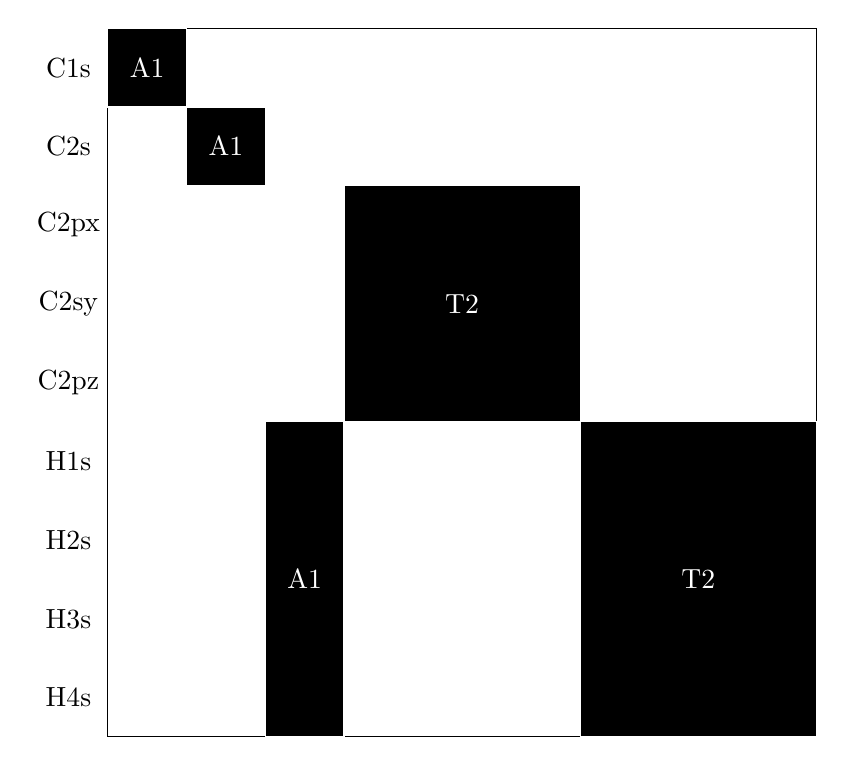
\begin{tikzpicture}
        \node[draw=none,
        rectangle, 
        minimum width = 1cm, 
        minimum height = 1cm
        ](r) at (-5cm,4cm) {C1s};
        \node[draw=none,
        rectangle, 
        minimum width = 1cm, 
        minimum height = 1cm
        ](r) at (-5cm,3cm) {C2s};
        \node[draw=none,
        rectangle, 
        minimum width = 1cm, 
        minimum height = 1cm
        ](r) at (-5cm,2cm) {C2px};
        \node[draw=none,
        rectangle, 
        minimum width = 1cm, 
        minimum height = 1cm
        ](r) at (-5cm,1cm) {C2sy};
        \node[draw=none,
        rectangle, 
        minimum width = 1cm, 
        minimum height = 1cm
        ](r) at (-5cm,0cm) {C2pz};
        \node[draw=none,
        rectangle, 
        minimum width = 1cm, 
        minimum height = 1cm
        ](r) at (-5cm,-1cm) {H1s};
        \node[draw=none,
        rectangle, 
        minimum width = 1cm, 
        minimum height = 1cm
        ](r) at (-5cm,-2cm) {H2s};
        \node[draw=none,
        rectangle, 
        minimum width = 1cm, 
        minimum height = 1cm
        ](r) at (-5cm,-3cm) {H3s};
        \node[draw=none,
        rectangle, 
        minimum width = 1cm, 
        minimum height = 1cm
        ](r) at (-5cm,-4cm) {H4s};
        
        \node[draw,
        rectangle, 
        minimum width = 9cm, 
        minimum height = 9cm
        ](r) at (0cm,0cm) {};

        \node[draw,
        rectangle, 
        color=white,
        fill=black,
        minimum width = 1cm, 
        minimum height = 1cm
        ](r) at (-4cm,4cm) {A1};

        \node[draw,
        rectangle,
        color=white, 
        fill=black,
        minimum width = 1cm, 
        minimum height = 1cm
        ](r) at (-3cm,3cm) {A1};

        \node[draw,
        rectangle,
        color=white,
        fill=black,
        minimum width = 1cm, 
        minimum height = 4cm
        ](r) at (-2cm,-2.5cm) {A1};

        \node[draw,
        rectangle, 
        color=white,
        fill=black,
        minimum width = 3cm, 
        minimum height = 3cm
        ](r) at (0cm,1cm) {T2};

        \node[draw,
        rectangle, 
        color=white,
        fill=black,
        minimum width = 3cm, 
        minimum height = 4cm
        ](r) at (3cm,-2.5cm) {T2};

    \end{tikzpicture}
    \caption{Symmetry assigned MOs}
\end{figure}


We implemented this procedure and tested this on methane with a minimal basis set.
We found that we could accurately assign the MOs and overall wavefunction of this
system with this method for the ground state, which was encouraging.
However, we encountered two problems. First was that the assignment of MOs did not
word as well for excited states.
The second was that for non-abelian groups, where there are some degenerate subspaces
such as E and T, this assignment also did not work for every case.

We discussed some ideas about using symmetry decomposition for the non-abelian 
point groups, but as this was a short study we decided that this might not be the
most prudent path. Additionally, this may have been a useful feature for testing
the benchmarking sets, but chlorophyll molecules would not be symmetric and so
type of assignment would probably not have worked. 
Hence, we could not confidently assign transitions from \dscf methods with this method.
We could still use the non-autonomous method of inspecting transition dipoles and
plots of MOs, but as mentioned above this would drastically increase the turnaround
time of including more systems in benchmarking, or other investigations.
Critically, it would also be impossible to fit a set of parameters to 'learn' transition
properties of systems, as will be discussed in the next chapter.

\subsubsection{Implications of Benchmarking Results}
\label{subsubsec:imp_of_benchmarking}

After considering this leading error, we can then make some statements on the
data presented.

Overall, the \dxtb method was inaccurate - far too inaccurate to be used as a 
viable method for transition properties of chlorophyll, or any other system.
The range of errors is quite large and there is also a significant systematic shift 
present. However the DFT methods, both the linear response and the \dscf methods,
are accurate at predicting excitation energies

We can try to pinpoint where the source of error might be from looking at methods
including in this benchmarking. First is that whilst the \dxtb method is inaccurate,
the sTDA-xTB results shows that a tight-binding approach that doesn't use full
linear-response can give very accurate results. Hence we could expect other similar
approaches to perform similarly well.

The next comparisons that could be made is whether the difference between 
linear-response and \dscf methods, or the difference between ab initio or 
semi-empirical methods, are the leading cause of error. Looking at the results 
for CAM-B3LYP/aug-cc-pVTZ, we can see that both the linear-response and \dscf 
results are fairly accurate. There are some outliers in the \dscf results, that 
we attribute to different transitions to excited states, however overall both 
have a majority of errors within a 0.5 eV range. Looking at the slightly lower
level theory DFT results, PBE0/Def2-SVP, we can see a marked decrease in accuracy.
Again, both linear-response and \dscf methods perform similarly, and so we attribute
the leading cause of error to be the electronic structure method, and not the response method.

We can continue this trend into the semi-empirical methods. Overall, these methods
performed much worse than the ab initio DFT methods, with the exception of the
sTDA-xTB method. There is still a relatively small difference between linear-response
xtb and \dxtb results, however both are fairly inaccurate and so this point is a
bit harder to justify. 

As the implementation of linear-response and \dxtb methods could use both the
SCC and non-iterative versions of the gfn-xtb methods (gfn1 and gfn0), we included
both in our test sets. We found that both are inaccurate, and there is a marked
drop when using gfn0. The systematic shift in the gfn0-\dxtb method is especially
bad. We conclude from this a response method based on out-of-the-box gfn-xtb would
not be viable - this is a conclusion that will be returned to in the following
chapter.

Overall, arguably the absolute worst was the eigenvalue difference method based
orbital energies (eigenvalues of the Hamiltonian diagonalisation) from the sTDA-xTB
method. To obtain these results, we used the available sTDA-xTB programs, that are
in two parts. The first part runs a version of xTB that provide molecular orbital
coefficients and energies for the sTDA program to then use to calculate the transition
properties.
on \code{xtb4stda} results. For these results we took the difference between
linear-response routine in the full sTDA-xTB method. This was the simplest method
that we included, and was a test to see whether the optimised electronic structure 
parameters were inherently good at predicting transition properties. As can be 
seen, this isn't the case, and so we could expect no real difference in a new
method if we started from this xtb method or a version of gfn-xtb. It seems that
the response method used can make up a large part of predicting transition properties
accurately.

The result that gfn-xtb based methods are not accurate is not unexpected. Tight-binding
methods in general are inaccurate methods are electronic interactions, due to not
including a large part of the electronic density. Additionally, they are highly
parameterised to the certain systems and problems. Whilst the gfn-xtb methods are
better than many other methods in this parameterisation, using a few pair-wise
parameters as possible to improve extensibility to systems outside the training
set, there will always be the problem that these parameters are trained on ground
state properties and not excited state properties. Whilst there was the possibility 
these parameters might have been accurate at both ground and excited state properties,
the results show that this just isn't the case.

\section{Conclusions and Further Work}
The two main hypotheses tested in this chapter have been whether a \dscf approach
to response properties can be as accurate as full linear-response or better, and
if a tight-binding based method could also be as accurate.

The answer to both of these are yes, but not at the same time, at least in the 
forms given in this chapter.

This is an encouraging step towards the overall thesis of this work. All of the
\dscf methods tested in this work have required much less cpu work, both in terms
of time and in memory, than the full linear-response methods. The difference is 
greater for the higher levels of theory, as this can amount to hours of cpu time
saved. For the tight-binding methods, this is not as stark until we start considering
much larger systems and problems.

The remaining issues and further work are outlined below.

\subsection{Symmetry}
\label{sec:dscf_symmetry}

The main problems as have been discussed have mainly been in assigning the correct
transition between different methods. A \dscf has not been as actively investigated
as TD-DFT methods, there are fewer developed tools for this kind of problem, much
less other programs or codes that could be used for reference. For example, many
TD-DFT codes can provide symmetry in their results, whereas it took alot of work
even to attempt to do so with \dscf. This would have been an unfinished problem 
going forward. However, due to the well defined $Q_y$ transition (discussed in the
following chapter), this may not be an issue for chlorophyll. But as further
work might include other systems, this would have been a recurring issue to be
solved. Additionally, it doesn't give much confidence to the results of the benchmarking.

Further work on this issue would be to return to this investigation. As reported, 
assigning ground state symmetries was successful, and much of the machinery required
was implemented.

\subsection{Embedding}
\label{subsec:dscf_embedding}

As reported in this chapter, these benchmarking results do not include any investigation
into how these methods would behave in an embedded system. This is more of an 
implementation problem than a theoretical problem for the majority of the methods
investigated, with the exception of the xtb based methods.
As implemented in \code{QCORE}, all of the DFT methods as well as the gfn1 based
method could have included embedding effects. This would be important to investigate
as we would have moved to more biological systems, where embedding effects can be
very important to include.
Further work on the remaining methods would have involved solving two problems. First would
be the formulation of embedding theory for gfn0, as this has not been investigated
before. We did perform some work on this area.

Second would be embedding the sTDA-xTB theory, which really would have required 
a deep investigation into the source code of this method. Given the scope of this
project, this was not a realistic consideration, especially for a relatively minor
part of the work.

\subsection{Scaling}
\label{subsec:dscf_scaling}

Whilst the \dscf results are promising in terms of accuracy and computational 
effort, this method may not be well suited for the issues discussed in the previous
chapter. The main issue is scaling up the volume of calculations that could reasonably
be done.
All of the semi-empirical methods used in this benchmarking all had a cpu walltime 
in the order of seconds, with very small memory requirements. Additionally, they
all could be run on a single core due to the larger overhead of serial calculations
as compared to the parallelisable routines - i.e. more time would be spent on running
SCF cycles or running functional code, which can only be run in serial, than on
constructing the Fock matrices or calculating integral values, which can be done in
parallel.
The opposite is true for the larger scale DFT calculations. Especially for the large
chlorophyll system, the memory requirements were much higher than the semi-empirical
methods. For example, using the \code{QCORE} implementation, all of the chlorophyll 
calculations required on the order of $10^2$ gb of memory, and would take ~90 minutes
of cpu walltime. This includes being parallelised over many cores (although not
nodes), all of which adds together to make a relatively expensive calculation. This
also means that it is entirely unfeasible to run these calculations on a desktop
computer.

This has two drawbacks. First, as said above, is the volume of calculations that
can be reasonably be done. This investigation used 27 individual chlorophylls, 
which would represent about half a days worth of supercomputer time. Expanding
this to a larger scale study of LHII, which can require up to thousands to hundreds
of thousands of calculations, would take weeks or months of computational time.
The first drawback then is that a study based on this method would not be repeatable
in the time frame of a single project. To discover a flaw or additional property 
that is needed, and so rerun all the calculations even twice or three times, would
take on the order of a year and so either be unfeasible or drastically reduce the
ability to test new ideas, given that nothing should be allowed to fail.
The second drawback is the lack of ease of use. As all calculations would have to
be run on a supercomputer, no small assays could be done on a local machine or desktop
computer. This is not a major problem, as many methods are unable to be run on a 
desktop computer, especially large scale DFT calculations. The problem here is that
the sTDA-xTB results, which were all run on a desktop computer, show that it is
possible to run these systems on smaller machines. It would be worth exploring
whether there are more, similar methods that could also achieve this, as this would
allow more researchers to be able to run larger systems without the previously needed
expense of time and energy, as well as allow for a quicker turnaround time on assays.
Additionally, it would also just allow more calculations to be run. This topic
is revisited in chapter \ref*{chap:LHII}.



